\section{Conclusion}\label{sec:rw:sgfd:synthese}
Après 20 années de recherche, la gestion de flux de données devient désormais suffisamment mature pour être appliquée massivement. Plusieurs produits commerciaux sont d'ailleurs maintenant utilisés en production. Toutefois, nous pouvons nous rendre compte que la complexité théorique de ces systèmes a été sous-estimée. De nombreux modèles ont été décrits pour représenter les flux de données et leurs traitements. Ces modèles sont encore remis en questions aujourd'hui au fur et à mesure du déploiement d'applications concrètes. Toutefois, les modèles sont bien souvent liés au système d'implémentation et certaines sémantiques d'exécutions ne sont pas claires. Ainsi, l'exécution de la même requête sur deux systèmes différents peut provoquer des interprétations différentes.

Nous avons vu que l'infrastructure des SGFD a reçu beaucoup d'attention en terme d'architecture, de tolérance aux fautes, d'intégration et de support du passage à l'échelle. Néanmoins, la compréhension de la sémantique des composants du SGFD est encore limitée. Ainsi, il est difficile d'intégrer deux SGFD, car ils ne partagent pas le même langage et que l'interprétation des langages peut être conflictuelle.

L'intégration des supports persistants reste ad hoc et souvent assistée par l'utilisateur. Les expressions de requêtes hybrides entre flux et relations persistantes sont faites par l'écriture de deux requêtes pour chaque système. Il est nécessaire d'avoir un langage capable d'exprimer les deux types d'interrogations, mais aussi de faire la jointure entre les deux mondes.

Les contributions sur l'optimisation de traitement des requêtes sont nombreuses. Mais peu de travaux~\cite{Galpin:snee,Kramer:semantics} proposent des optimisations de plan de requêtes similaires aux SGBD (optimisation logique puis physique). Dû au manque de connaissances sur les équivalences de requêtes, seules les règles simples telles l'application de projections au plus près des sources sont faites dans l'optimisation logique. Il est nécessaire d'avoir une \textit{recherche d'optimisation plus approfondie} sans intervention de l'utilisateur, ce qui est limité en l'état.

\newpage
\quad

\vspace{2.3\baselineskip}
\begin{flushright} \huge Présentation des contributions \end{flushright}
\vspace{1.7\baselineskip}

Cette thèse souhaite adresser le problème de l'observation de système. Le constat est que les systèmes produisent des données hétérogènes en terme de schéma ainsi qu'en terme de dynamisme. De plus, nous souhaitons que ce système d'observation soit flexible pour pouvoir s'adapter aux différents besoins des utilisateurs.

Notre contribution se focalise sur trois points principaux :
\begin{itemize}
 \item[\textbf{Modélisation}] : Création d'Astral, algèbre de traitement des requêtes continues sur flux et relations temporelles. En particulier, les définitions sont indépendantes du système d'implémentation. Cela permet l'optimisation et la médiation de systèmes. Cette algèbre est présentée dans le chapitre~\ref{chap:contrib:astral}. Son expressivité ainsi que la démonstration d'équivalences de requêtes sont présentées dans le chapitre~\ref{chap:validation:expressivite}.
 \item[\textbf{Exécution}] : Mise en œuvre de l'intergiciel Astronef pour construire et exécuter efficacement les requêtes exprimées avec l'algèbre Astral. Ce moteur intègre un constructeur de plan de requête sélectionnant un assemblage de composants efficace pour exécuter une expression algébrique. Cette mise en œuvre est développée dans le chapitre~\ref{chap:contrib:astronef}.
 \item[\textbf{Persistance}] : Conception de l'extension Asteroid permettant l'intégration des requêtes continues sur flux et des requêtes sur support relationnel persistant. Ceci permet de gérer la représentation du système observé ainsi que l'historisation des données dynamiques. Il devient possible d'interroger via le même langage, les données temps réel et persistantes. Le support formel de cette intégration est effectué par Astral et sa mise en œuvre par Astronef. Ces travaux sont présentés dans le chapitre~\ref{chap:contrib:asteroid}.
\end{itemize}

Ces contributions sont validées par expérimentations dans les chapitres~\ref{chap:valid:domvision} et~\ref{chap:valid:perfs}. De plus, nous proposons une extension permettant de \textbf{personnaliser} les résultats des requêtes dans le chapitre~\ref{chap:prefs}. Ainsi, face à la masse de données auquel l'utilisateur est confronté, il sera en mesure de réduire le volume de données à restituer selon ses préférences.

Grâce à l'ensemble de ces contributions, il devient possible de mettre en œuvre un système d'observation générique applicable sur un large ensemble de données. L'utilisateur exprime des requêtes dans le langage algébrique Astral. Les requêtes sont ensuite exécutées par Astronef-Asteroid. 

\begin{figure}[ht]
	\centering
	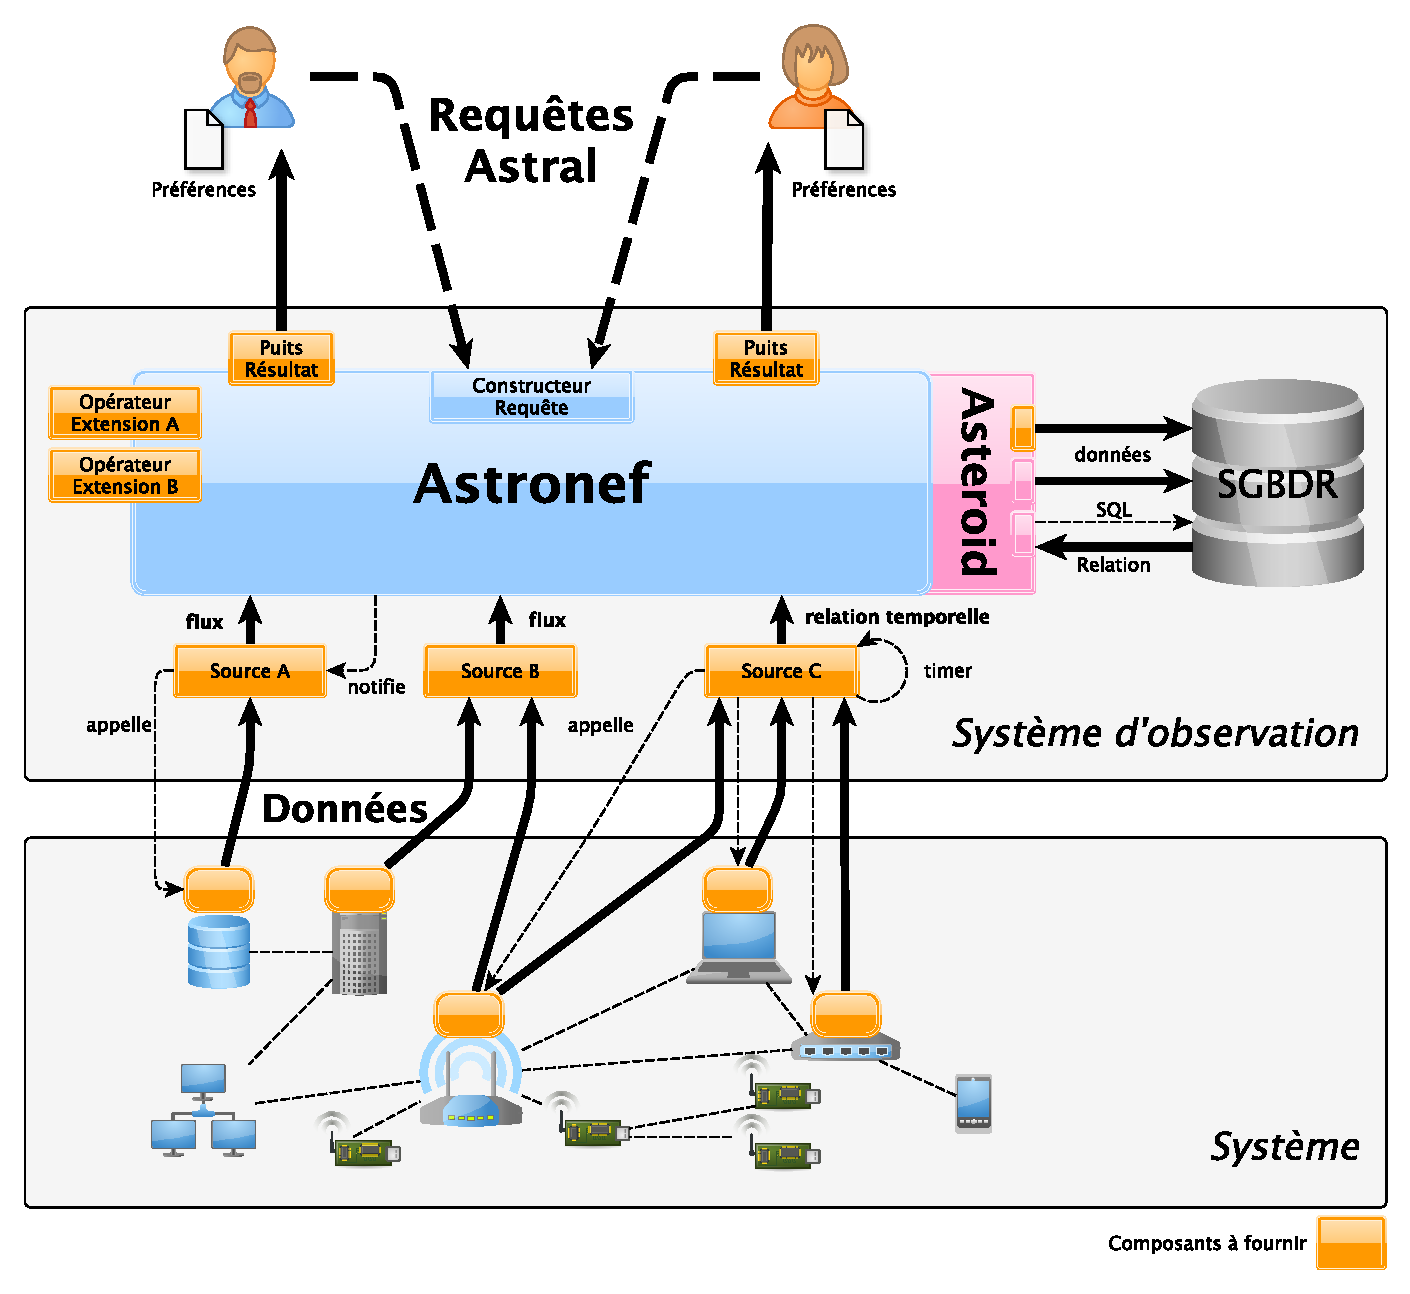
\includegraphics[width=\textwidth]{contrib-global}
	\caption{Présentation des contributions de cette thèse}
\end{figure}
